\documentclass[french]{article}
\usepackage[T1]{fontenc}
\usepackage[french]{babel}
\usepackage[utf8]{inputenc}
\usepackage{a4wide}
\usepackage{amssymb}
\usepackage{amsmath}
\usepackage{listings}
\usepackage{graphicx}
\usepackage{xcolor}


% --Listings OCaml-- %
\definecolor{codegray}{rgb}{0.5,0.5,0.5}
\definecolor{backcolour}{rgb}{0.95,0.95,0.92}

\lstdefinelanguage{Ocaml}{
    keywordstyle=\color{orange},
    morekeywords={
        let,
        fun,
        ref,
        in
    },
    numbers=none,
    basicstyle=\ttfamily\footnotesize,
    breakatwhitespace=false,
    tabsize=4
}

% --Listings RAT-- %
\lstdefinelanguage{ratcode}
{
    keywordstyle=\color{orange},
    morekeywords={
        int,
        define,
        loop,
        break,
        bool,
        rat,
        if,
        else,
        call,
        return
    },
    sensitive=false,
}

% --JUGEMENTS-- %
\newcommand{\jugementPointeur}{
        \dfrac{\sigma \vdash id : \tau}
              {\sigma \vdash *id : \tau, \pi} \text{où }\pi \text{ est la marque.}\\
        \text{Par suite, } \tau_r \text{ est l'environnement de type et de marque.}\\
        \text{Les jugements de typages sont alors inchangés, simplement on peut remplacer}\\
        \text{pour les variables id par *id en suivant le typage ci-dessus.}
        }

\newcommand{\jugementElseOpt}{
        \dfrac{\sigma \vdash E : \text{bool} \hspace*{10pt} \sigma, \tau_r \vdash \text{BLOC} : \text{void}}
              {\sigma, \tau_r \vdash \text{if } E \text{ BLOC} : \text{void}, []}
        }

\newcommand{\jugementTernaire}{
        \dfrac{\sigma \vdash E : \text{bool} \hspace*{10pt} \sigma \vdash E_1 : \tau \hspace*{10pt} \sigma \vdash E_2 : \tau }
              {\sigma \vdash (E \text{ ? } E_1 : E_2) : \tau}
        }

\newcommand{\jugementLoop}{
        \dfrac{\sigma, \tau_r \vdash \text{BLOC} : \text{void}}
              {\sigma, \tau_r \vdash \text{loop} \text{ BLOC} : \text{void}, []}
        }
\newcommand{\jugementLoopId}{
        \dfrac{id::\sigma, \tau_r \vdash \text{BLOC} : \text{void}}
              {\sigma, \tau_r \vdash \text{define id : loop} \text{ BLOC} : \text{void}, []}
        }

\newcommand{\jugementIncrementPost}{
        \dfrac{\sigma \vdash id : \text{Int}}
              {\sigma \vdash \text{id}++ : \text{Int}}
        }

\newcommand{\jugementIncrementPre}{
        \dfrac{\sigma \vdash id : \text{Int}}
              {\sigma \vdash ++\text{id} : \text{Int}}
        }

\begin{document}


\title{\textbf{Traduction des Langages}}
\author{Quentin \textsc{Fraty}\\
        Nathan \textsc{Maillet}}
\date{}

\maketitle

\section{Introduction}
\paragraph*{Dans la continuité des cours / TDs / TPs effectués en cours de Traduction des Langages, un projet de développement de compilateur
a été réalisé. Le langage d'origine choisi fut le Rat, un langage très limité en nombre d'instructions différentes réalisables.\\
Le langage cible, quand à lui était un pseudo langage assembleur pouvant être exécuté directement à travers un programme spécialisé.}
\paragraph*{Comme nous allons le voir tout au long de ce rapport, une grande variété de fonctionnalités ont été ajoutées au langage Rat,
avec comme objectif de le rendre plus complet, et plus proche des langages bas niveau manipulés aujourd'hui (Rust, C).\\
Notamment, voici les différentes fonctionnalités implémentées et opérationnelles, qui seront abordées~:
\begin{itemize}
        \item Ajout des pointeurs, et accès par référence à des variables.
        \item Ajout du côté optionel au bloc else d'une conditionnelle.
        \item Ajout des expressions ternaires.
        \item Ajout des boucles `à la Rust'.
\end{itemize}}
\,
\paragraph*{Voici ensuite les fonctionnalités non demandées implémentées~:
\begin{itemize}
        \item Ajout de la surcharge de fonctions (même nom, différents types de paramètres).
        \item Ajout d'instructions pour l'incrémentation rapide (v++, ++v, v+=42).
        \item Ajout d'une backtrace en cas d'erreur.
\end{itemize}}


\section{Mutation de \emph{tds.ml} en \emph{mtds}}
\paragraph*{La première étape avant de se lancer sur le projet était de modifier \emph{tds.ml} afin de ne plus le modifier,
même si par la suite nous voulions modifier notre raisonnement, comme par exemple ce qui est arrivé sur les pointeurs (cf 3.Pointeurs).}
\subparagraph*{\emph{mtds.ml} a donc pour but de généraliser \emph{tds.ml}. Nous sommes donc passés d'Identifiants \emph{string}
en un type paramétré \emph{'a}, ce qui explicite l'aspect monadique de la tds sans pour autant contraindre le module, ce qui aurait été un apport négligeable en OCaml 4
pour le cadre dans lequel nous avons codé (pas de gestion très poussée des exceptions ou de foncteurs).
Par ailleurs, dans le cas où nous voulions plus tard modifier notre langage rat il aurait été intéressant d'avoir parétrer \emph{tds.ml} pour ajouter, par exemple,
des casts de type s'ils étaient implémentés.} % ou si nous voulions donner la possibilité au codeur d'expliciter les kinds de ses types 

\section{Pointeurs}
\paragraph*{Le choix lié au traitement des pointeurs revient a se demander comment nous considérons les mots \emph{int * a}.
Alors que nous pouvons considérer une variable de type \emph{Pointeur(int)} et d'indentifiant \emph{a}, il nous semblait plus
famillier de voir ça comme une variable de type \emph{int} et d'identifiant \emph{Pointeur(a)}.}
\paragraph*{Cela nous a mené vers une première tentative qui était devenue trop rigide pour les manipulations que nous voulions faire avec les pointeurs.
C'est alors que nous avons changé pour une troisième façon de voir les choses~: c'est tout simplement une variable avec un type \emph{int}, une
\emph{marque} \emph{Pointeur(Neant)} et un symbole \emph{a}, la \emph{marque} et le symbole formant l'identifiant.}
\subparagraph*{Une marque représente alors le niveau de pointeurs et n'est ni lié au type ni au symbole. Avec cette représentation, nous avons alors pu
nous lancer sereinement dans l'implémentation des pointeurs, avec une modification de tous nos jugements de typages suivant celui ci-dessous~:\\}
\(\jugementPointeur\)

\paragraph*{Pour les ASTs, seul les ajouts lexicaux ont été inclus sans nouvelle modification.}

\paragraph*{On peut noter que dans l'implémentation des pointeurs que nous avons fait, il est possible d'affecter un pointeur à la déclaration.
Par exemple, est possible~:}
\,
\begin{lstlisting}[language=ratcode]
int a = 5;
int *b = &a;
\end{lstlisting}

\section{Bloc else optionnel}
\paragraph*{Grâce à la façon choisie initialement pour traiter les blocs conditionnels, il fut assez simple d'implémenter cette fonctionnalité.
En effet, lors du parsing, il suffit de créer un \emph{AstSyntax.Conditionnelle} avec un bloc else vide, et de le traiter comme un bloc conditionnel classique.
Le typage est inchangé, et le code produit est le même que si le bloc else était présent.}
\paragraph*{Cette solution permet de minimiser la redondance de code, et de ne pas avoir à traiter le bloc else comme un cas particulier, avec
un ajout d'un else dans la passe de génération de code dans tous les cas. Cela n'a aucun impact sur l'exécution du programme.}
\paragraph*{Au niveau du jugement de typage, dans la mesure où le bloc else est vide, celui-ci peut être résumé comme suit:}
\[\jugementElseOpt\]

\section{Conditionnelle ternaire}
\paragraph*{Cette fonctionnalité ajoutée au langage Rat a nécessité de créer un nouveau type d'expression, \emph{AstSyntax.Ternaire}.
Tout d'abord, il a fallu modifier la grammaire pour accepter cette nouvelle expression.}
\subparagraph*{Au niveau du lexer, il a fallu ajouter le symbole \texttt{?} et \texttt{:} dans la liste des symboles à accepter. Au niveau du parser, il a fallu ajouter une règle pour accepter cette nouvelle expression~:}
\,% les listings sont kssé
\begin{lstlisting}
| PO e1=e QMARK e2=e COLON e3=e PF  {Ternaire (e1,e2,e3)}
\end{lstlisting}

\paragraph*{Ensuite, les différentes passes du compilateur ont successivement vérifié les choses suivantes~:
\begin{itemize}
        \item La conformité des identifiants utilisés dans les trois expressions de la conditionnelle ternaire.
        \item Le fait que la premiere expression soit bien booléenne, et que les deux autres soient de même type. Cela peut être résumé par le jugement de typage suivant~:
\end{itemize}}
\[\jugementTernaire\]
\paragraph*{Enfin, la génération du code associé à un ternaire se rapproche à celui d'une instruction conditionnelle, 
dans la mesure où la valeur mise en sommet de pile est celle de l'une des deux expressions~: l'utilisation de jump est alors nécessaire.}
\,
\begin{lstlisting}[language=Ocaml]
| AstType.Ternaire(e1, e2, e3) -> 
      let labElse = getEtiquette ()
      and labEndIF = getEtiquette () in
      ast_to_tam_expression e1
      ^ jumpif 0 labElse
      ^ ast_to_tam_expression e2
      ^ jump labEndIF
      ^ label labElse
      ^ ast_to_tam_expression e3
      ^ label labEndIF
\end{lstlisting}

\section{Loop à la Rust}
% Manque de parler de si on autorise ou non une variable id si id est déjà pris pour une boucle !
% D'ailleurs, giveID ne risque pas de donner un nom de variable sans faire exprès ? On pourrait ajouter '+' dans l'id

\paragraph*{Les loop à la rust sont une extension du langage Rat qui permet de créer des boucles infinies,
avec la possibilité d'en sortir à l'aide du mot clé \texttt{break} 
et de terminer prématurément une itération à l'aide du mot clé \texttt{continue}.}
\paragraph{Face aux difficultés que celle-ci a pu nous poser, il nous a semblé important de commenter nos choix effectués pour obtenir une grammaire cohérente.
En effet, en reprenant la syntaxe du sujet pour les boucles nommées (l : loop{bloc}), des problèmes d'ambiguîté empêchaient Menhir de comprendre correctement la grammaire.
Comme le montre la capture d'écran ci-après, l'erreur ne nous indiquait pas la source de l'ambiguîté. Mais même en analysant les logs de compilation, nous ne sommes
pas parvenus à déterminer l'origine de ces conflits, empêchant un fonctionnement de notre compilateur:\\}
\begin{center}
        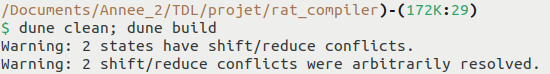
\includegraphics[scale=0.5]{shift_reduce.png}
\end{center}
\paragraph{Pour éviter cette erreur, nous avons fait le choix de modifier la grammaire d'une telle manière que les règles d'écriture d'une boucle ne pourraient
plus êtres ambiguês pour Menhir. Ainsi, voici comment nous avons choisi qu'une boucle nommée devait s'écrire: } % TODO: ça s'affiche pas mdr
\begin{lstlisting}[language=ratcode]
        define l : loop {bloc};
\end{lstlisting}
\paragraph{Par l'ajout du mot-clé \texttt{define} en début de règle, et d'un point virgule en fin, l'ambiguîté est alors levée, et le compilateur fonctionne 
correctement.}
\paragraph*{Comme nous allons le voir, toute la complexité des boucles à la rust est liée à la gestion des labels, qui est exclusivement gérée par la passe de gestion d'identifiants.\\
Tout d'abord, il a été choisi de créer un nouveau type de données insérable dans la table des symboles.}
\subparagraph*{En effet, il est nécessaire de stocker les informations liées à une boucle pour pouvoir la terminer, ou la recommencer
lorsqu'un \texttt{break} ou \texttt{continue} est utilisé.\\
Cependant, et ce comme énoncé dans le sujet, il fallait donner la possibilité à l'utilisateur d'imbriquer des fonctions de même label.\\
Pour ce faire, ce nouvel élément de la TDS associe à un label une InfoBoucle, qui contient en réalité une liste d'informations (couple de \emph{string}) associées à ce label.\\
Cela permet de prendre en compte le cas où deux boucles de même label sont imbriquées, et de pouvoir les distinguer. \\} % Espacement voulu
\subparagraph*{Un deuxième choix de conception que nous avons fait est sur les identifiants de boucles dans la TDS.\\
Tout d'abord, à toute boucle est associé un identifiant pour la TDS~: soit celui donné par l'utilisateur, soit un identifiant uniqué généré par le compilateur
de manière analogue à la génération de labels lors de la passe de génération de code.}
\,
\begin{lstlisting}[language=Ocaml]
let giveID = 
  let num = ref 0 in
  fun () ->
    num := (!num)+1 ;
    "id"^((string_of_int (!num)))
\end{lstlisting}
\paragraph*{Ensuite, l'information associée à une boucle est le couple (label de début, label de fin), qui sont générés par le compilateur à partir du label précédent. \\
Ainsi, lorsque deux boucles de même label sont utilisées, l'\emph{infoboucle} associée au label est une liste de couples 
(label de début, label de fin), dont la tête est le couple associé à la plus imbriquée.
En exploitant l'aspect récursif des fonctions, il est possible de récupérer le label de début/fin de la boucle la plus imbriquée facilement,
ce qui est la logique choisie pour le \texttt{break} et le \texttt{continue}.}\,
\subparagraph*{De plus, il fallait donner la possibilité à l'utilisateur de ne pas utiliser de labels pour les \texttt{loops}, \texttt{break} et \texttt{continue}. Le comportement
choisi devait alors être que tout \texttt{break} / \texttt{continue} aurait un effet sur la boucle courante, et dans le cas d'imbrication de boucles, celle la 
plus imbriquée.\\
Pour pouvoir implémenter cela, il a été choisi de \emph{décorer l'arbre} avec l'infoboucle associée à la boucle courante pour pouvoir associer au \texttt{break} / \texttt{continue}
la bonne boucle.}
\paragraph*{Suite à cette passe, celle de typage est comparativement triviale, dans la mesure où celle-ci revient à une analyse
du typage d'un bloc. Voici les jugements de typage associé~:}
 \[\jugementLoop \text{ et } \jugementLoopId\]
\paragraph*{La passe de placement mémoire, de manière analogue, revient à analyser le placement mémoire des variables du bloc de la boucle.}
\paragraph*{En revanche, la passe de génération de code s'avérera poser des difficultés que nous n'avions pas anticipé. En effet, chaque itération de boucle doit
écrire ses variables locales au même endroit, ce qui pose des problèmes lorsqu'un \texttt{break} ou un \texttt{continue} sont utilisés: alors que le TantQue
implémenté en Rat assurait l'exécution entière de son bloc courant avant de se finir, ce n'est pas le cas de la boucle à la Rust. \\
Ainsi, en imaginant qu'après un \texttt{break} il y a une déclaration de variable (et donc un push de la pile), il s'avérait nécessaire
d'avoir le déplacement dans la boucle jusqu'au \texttt{break} en tant que paramètre hérité (décoration d'arbre). Cependant même avec une telle chose, 
le cas d'imbrication de boucle ne semblait pas traitable facilement de manière pure, dans la mesure où un \texttt{break} peut aussi faire sortir d'une boucle moins imbriqué, comme dans 
l'exemple suivant~:}

\, % les listings sont kssé
\begin{lstlisting}[language=ratcode]
main {
    int x = 3;
    define l : loop {
        x++;
        loop {
                int y = 5;
                break l;
                bool z = true;
        };
        rat r = [3/2];
    };
}
\end{lstlisting}
\paragraph*{Ici, il faudrait se rappeler au niveau du \texttt{break} l que cela revient à pop 1, et pas 2 ou 3 qui serait obtenu si on prenait toutes les déclarations réalisées.\\
N'ayant pas de solution simple à ce problème et par manque de temps, il a été choisi de ne \emph{pas} pop le contexte d'une boucle en cas de \texttt{break} ou \texttt{continue}.
Ce choix, bien que semblant fonctionner, peut poser des problèmes de pile. En effet, si un \emph{print} survient après la boucle, il sera en haut de ce qui n'a pas été nettoyer dans la pile.
Dans le cas où nous sommes en haut de la pile, ce \emph{print} va donc load dans le tas ou échouer, ce qui n'aurait pas eu lieu avec une pile mieux gérée.}

\section{Surcharge de fonctions}
\paragraph{Nous avons décidé d'implémenter en plus dans notre projet une notion évoquée lors de l'examen écrit de TDL~: la surcharge de fonctions.
Ce concept autorise l'existence dans un même programme de fonctions ayant le même nom, mais une signature différente au niveau des paramètres.}
\paragraph{Pour pouvoir accepter la surcharge de fonctions, il a tout d'abord fallu modifier le type InfoFun, dans la mesure où l'on devait connaître 
toutes les différentes signatures qui pouvaient êtres associées à un nom. Ainsi, une InfoFun contient désormais une liste de signatures, chacunes représentées sous
la forme d'une liste de paramètres/retour.}
\paragraph{Ce changement implique le fait de modifier l'analyse de gestion des identifiants des fonctions dans la passe associée~: l'exception DoubleDéclaration
ne doit désormais être levée que si l'on essaie de définir une fonction avec le même nom et les mêmes types de paramêtres.}
\paragraph{La dernière modification à effectuer sur le compilateur consiste en la résolution de surcharge lors de l'appel d'une fonction. Cela est réalisé
dans la passe de Typage, où les types des paramètres utilisés sont comparés aux différentes signatures connues de la fonction appelée. Ainsi, la surcharge
de fonction est belle et bien fonctionnelle.}

\section{Incréments}
\paragraph*{Il a été choisi d'implémenter dans le langage Rat de nouvelles fonctionnalités qui puissent êtres traitées au niveau du parseur. C'est pourquoi
l'incrémentation comme en C (variable++ et ++variable) a été partiellement ajoutée~: contrairement à C, ces deux éléments sont considérés comme
des instructions à part entière et ne peut être utilisé dans une expression. Voici les lignes associées dans le fichier Parser~:}
\,
\begin{lstlisting}
| PLUS PLUS n=r PV 
{Affectation (n,Binaire (Plus,Identifiant n,Entier 1))}
| n=r PLUS PLUS PV 
{Affectation (n,Binaire (Plus,Identifiant n,Entier 1))}
\end{lstlisting}

\subparagraph*{De manière similaire, l'opérateur '+=' a été ajouté au langage Rat, et ce grâce à une transformation directement dans le parseur~:}
\,
\begin{lstlisting}
| n=r PLUS EQUAL e1=e PV 
{Affectation (n,Binaire (Plus,Identifiant n,e1))}
\end{lstlisting}

\paragraph*{Ainsi, dans la mesure où ces instructions sont `converties' en combinaisons d'éléments simples compris par notre compilateur, aucune passe n'a
à être adaptée pour prendre en compte ces opérations.}
\paragraph*{Les jugements de typages liés à ces instructions peuvent alors être obtenu par déduction de ceux sur les affectations d'entiers~:}
\[\jugementIncrementPost \text{ et } \jugementIncrementPre\]

\section{Affichage des erreurs}
\paragraph*{La génération de backtrace est la dernière fonctionnalité optionnelle que nous avons ajouté à notre compilateur Rat. \\
Celle-ci permet à un développeur de savoir précisément à quelle instruction de quel bloc se situe l'erreur empêchant la compilation. 
Voici par exemple la backtrace générée~:}

\begin{center}
        \lstinputlisting[language=ratcode]{factrecError.rat}
\end{center}
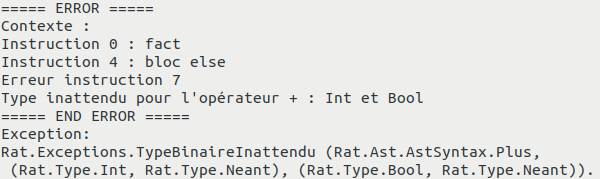
\includegraphics[width=\textwidth]{backtrace.png}

\paragraph*{Ce résultat utilise le concept de décoration d'arbre, comme réalisé pour d'autres fonctionnalités~: après la passe de gestion des identifants,
à chaque instruction est rajouté un contexte. Il s'agit d'une liste de couple (numéro de ligne, nom du bloc) représentant avec précision la localisation
de chaque instruction dans le code. Ainsi, toute erreur levée fait désormais appel à notre fonction `afficher\_erreur' prenant en paramètres
un contexte,une exception et son numéro de ligne, et l'affichant comme montré précédemment.}

\section{Conclusion}
% Bon recul sur les difficultés rencontrées et améliorations éventuelles
% Améliorations éventuelles :
% On autorise les pointeurs dans les paramètres mais pas en retour
% Effacer les lignes de ce message UNIQUEMENT lorsque qu'elles ont été traitées
\paragraph*{Différentes améliorations pourraient être apporté à ce compilateur.
Au-delà du fait que nous ne traitons pas le cas de l'optimisation du code source, les difficultés mentionées tout au long de ce rapport mettent en évidence les améliorations possibles suivantes~:
\begin{itemize}
        \item Les initiatives prises au niveau du parsing mettent en évidence un problème qui pourrait être corrigé.
        \item Les pointeurs ne sont effectif que sur des variables et retours. Il peut pourtant être très
        intéressant d'avoir des pointeurs sur fonction qui impliqueraient une gestion du LB part le code assembleur mais permettrait
        de faire facilement des fonctions d'ordres "supérieurs" (dans l'absolu on gèrerait des pointeurs et non des fonctions).
\end{itemize}}
\paragraph*{De plus, et ce malgré les apports demandés par le sujet et nos initiatives personnelles, le langage Rat reste très limité. Voici les différentes 
fonctionnalités que nous aurions désiré implémenter mais n'avons pas pu, faute de temps~:
\begin{itemize}
        \item Fonctions d'ordre supérieur
        \item Les modules
\end{itemize}}
\paragraph*{Enfin, et ce au niveau du compilateur en lui-même, il aurait été intéressant d'aborder l'optimisation de compilation, à travers par exemple la
suppression de code mort (toute instruction après un retour dans un même bloc).}
\end{document}
